\documentclass[border=3pt]{standalone}
\usepackage{palatino}
\usepackage[T1]{fontenc}
\usepackage[utf8]{inputenc}
\usepackage{amsmath,amssymb}
\usepackage{tikz}
\usetikzlibrary{arrows.meta,shapes,positioning,decorations.pathreplacing,calc}
\usepackage{xcolor}

% Misma paleta que latent_reasoning_schematic.tex, para que los dos esquemas
% del poster (eje K y eje c) se lean como parte de la misma familia visual.
\definecolor{lrGray}{HTML}{6E6D66}
\definecolor{lrBlue}{HTML}{444D8A}
\definecolor{lrBlueDk}{HTML}{2E3566}
\definecolor{lrRasp}{HTML}{B0485F}
\definecolor{lrRaspDk}{HTML}{8F3A4D}
\definecolor{lrInk}{HTML}{33322F}
\definecolor{lrLabel}{HTML}{5C5B57}

\begin{document}
  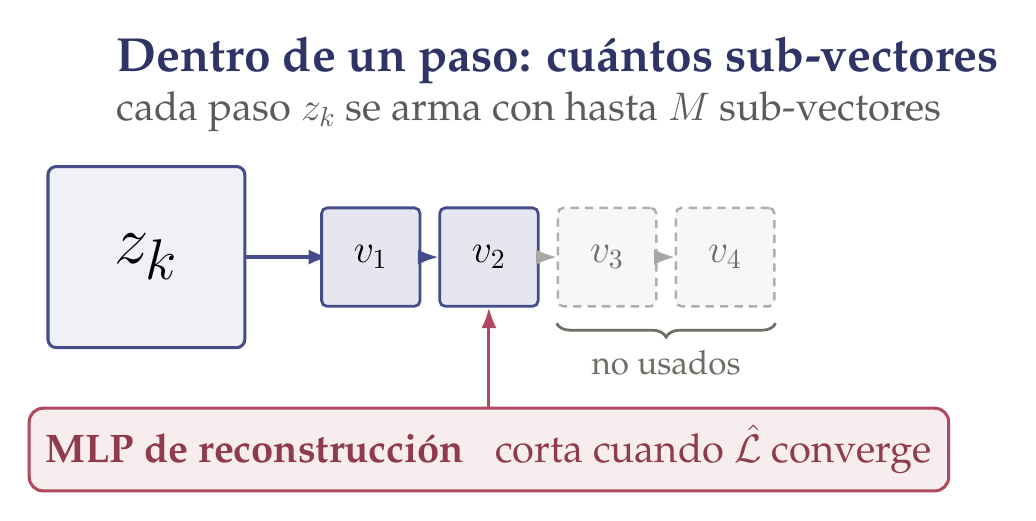
\begin{tikzpicture}[
      font=\rmfamily,
      >={Latex[length=2.6mm]},
      stepbox/.style={rounded corners=3pt, minimum width=2.5cm, minimum height=2.3cm,
                  align=center, inner sep=2pt,
                  draw=lrBlue, line width=1.1pt, fill=lrBlue!8},
      subv/.style={rounded corners=2pt, minimum width=1.25cm, minimum height=1.25cm,
                  inner sep=1pt, draw=lrBlue, line width=1.0pt, fill=lrBlue!14,
                  font=\Large},
      subvskip/.style={rounded corners=2pt, minimum width=1.25cm, minimum height=1.25cm,
                  inner sep=1pt, draw=lrGray!55, line width=0.9pt,
                  dash pattern=on 3pt off 2.2pt, fill=black!3, font=\Large,
                  text=lrGray},
      title/.style={anchor=west, font=\LARGE\bfseries},
      sub/.style={anchor=west, font=\Large, text=lrLabel},
    ]

    % ---------- título ----------
    \node[title, text=lrBlueDk] at (-6.9,2.35) {Dentro de un paso: cu\'antos sub-vectores};
    \node[sub]                  at (-6.9,1.7)  {cada paso $z_k$ se arma con hasta $M$ sub-vectores};

    % ---------- paso de referencia (izquierda) ----------
    \node[stepbox] (zk) at (-6.4,-0.15) {\Huge\itshape$z_k$};

    \draw[->, lrBlue, line width=1.2pt] (zk.east) -- ++(1.05,0);

    % ---------- sub-vectores dentro del paso ----------
    \node[subv]     (v1) at (-3.55,-0.15)  {$v_1$};
    \node[subv]     (v2) at (-2.05,-0.15)  {$v_2$};
    \node[subvskip] (v3) at (-0.55,-0.15)  {$v_3$};
    \node[subvskip] (v4) at ( 0.95,-0.15)  {$v_4$};

    \draw[->, lrBlue, line width=1.0pt] (v1)--(v2);
    \draw[->, lrGray!60, line width=0.9pt] (v2)--(v3);
    \draw[->, lrGray!60, line width=0.9pt] (v3)--(v4);

    % ---------- llave: sub-vectores no usados ----------
    \draw[decorate, decoration={brace, amplitude=5pt, mirror}, lrGray, line width=1.0pt]
      ([yshift=-2mm]v3.south west) -- ([yshift=-2mm]v4.south east)
      node[midway, below=6pt, font=\large, text=lrGray] {no usados};

    % ---------- MLP de reconstruccion ----------
    \node[rounded corners=5pt, draw=lrRasp, line width=1.1pt, fill=lrRasp!10,
          anchor=north, minimum width=9.6cm, minimum height=1.05cm, inner sep=6pt,
          text=lrRaspDk, font=\Large] (mlp) at (-2.05,-2.05)
      {{\bfseries MLP de reconstrucci\'on} \; corta cuando $\hat{\mathcal{L}}$ converge};

    \draw[->, lrRasp, line width=1.1pt] (mlp.north) -- (v2.south);

  \end{tikzpicture}
\end{document}
